\documentclass{article}
\usepackage[utf8]{inputenc}
\usepackage{multicol}
\usepackage{amsmath}
\usepackage{float}
\usepackage{epsfig,graphicx}
\usepackage{xcolor,import}
\usepackage{subcaption}
\usepackage[font=small,labelfont=bf]{caption}
\usepackage{siunitx}
\usepackage[german]{babel}
\usepackage{textcomp}
\usepackage{mathtools}

\begin{document}


\thispagestyle{empty}
			\begin{center}
			\Large{Fakultät für Physik}\\
			\end{center}
\begin{verbatim}


\end{verbatim}
							%Eintrag des Wintersemesters
			\begin{center}
			\textbf{\LARGE SOMMERSEMESTER 2015}
			\end{center}
\begin{verbatim}


\end{verbatim}
			\begin{center}
			\textbf{\LARGE{Physikalisches Praktikum II}}
			\end{center}
\begin{verbatim}




\end{verbatim}

			\begin{center}
			\textbf{\LARGE{PROTOKOLL}}
			\end{center}
			
\begin{verbatim}





\end{verbatim}

			\begin{flushleft}
			\textbf{\Large{Experiment 2: Elektrische Schwingungen}}\\
							%Experiment Nr. und Titel statt den Punkten eintragen
			\LARGE{}	
			\end{flushleft}

\begin{verbatim}

\end{verbatim}	
							%Eintragen des Abgabedatums, oder des Erstelldatums des Protokolls
			\begin{flushleft}
			\textbf{\Large{Datum:}} \Large{20.03.2015}
			\end{flushleft}
			
\begin{verbatim}
\end{verbatim}
							%Namen der Protokollschreiber
		\begin{flushleft}
			\textbf{\Large{Grafendorfer Erik}} 
			\end{flushleft}

\begin{verbatim}


\end{verbatim}
							%Kurstag und Gruppennummer, zb. Fr/5
			\begin{flushleft}
			\textbf{\Large{Kurstag/Gruppe:}} \Large{FR/1}
			\end{flushleft}

\begin{verbatim}






\end{verbatim}
							%Name des Betreuers, das Praktikum betreute.
			\begin{flushleft}
			\LARGE{\textbf{Betreuer:\Large{Fuith}}}		
			\end{flushleft}
			
\section{Aufgabenstellung}
An Kondensatoren und Spulen in verschiedenen Serienschaltungen sollen die Effekte eines Schwingkreises untersucht werden, wie das Abklingen, das durch Energieverlust an Leitungswärme entsteht, erzwungene Schwingungen, sowie Schwebung mit einem zweiten Schwingkreis.
\section{Theorie}
Ein elektrischer Schwingkreis aus einem Kondensator mit einer Kapazität C und einer Spule mit einer Induktivität L in einem Stromkreis mit der Spannung U lässt sich mit der gleichen Differentialgleichung beschreiben wie ein mechanischer Oszillator:

\begin{equation}
\label{HarmOsz}
L\frac{d^2q}{dt^2}+RI-\frac{q}{C}=0
\end{equation}

Als Lösung wählen wir dabei 
\begin{equation}
\label{Schwingungsgleichung}
\frac{q(t)}{C}=U(t)=U_{0}\cdot e^{\delta t}\cdot \cos{\omega t}
\end{equation}

Für ganzzahlige Vielfache der Periodendauer T erhalten wir das wichtige Ergebnis:
\begin{equation}
\label{LogarithmDekr}
\Lambda=\log{\frac{U(nT)}{U((n+1)T}}=delta T
\end{equation}
$\omega_{0}$=$\sqrt{\omega_{0d}^2+\delta^2}$\\
Q=$\frac{\omega_{0d}}{2\delta}$ \\
$$R=\delta \cdot 2L$$ \\
\section{Aufbau}
Ein Schwingkreis bestehend aus einem Kondensator, einer Spule und einem fallweise geschalteten Widerstand wird durch einen Funktionsgenerator mit variablen Spannungen angeregt und seine Schwingung an einem 2-Kanal Oszilloskop beobachtet. Später wird ein identischer, weiterer Schwingkreis über eine Kondensatorkaskade angekoppelt und zur Interaktion mit dem ersten gebracht.
\section{Durchführung}
Es wurde immer der Kondensator C2 verwendet und fallweise ein Widerstand von 2.2 $\pm 10\% \Omega$.
\section{Ergebnisse}
\subsection{Freie Schwingungen}
$$T=2 \cdot 10^{-4}s$$
\subsubsection*{Ohne Dämpfung}
\begin{center}
$\delta$= 272 $\pm$ 3\\
$\omega_{0d}=(3.1416\cdot \pm 0.0001)10^4 s^{-1}$\\
$\omega_{0}=(3.1417\cdot \pm 0.0001)10^4 s^{-1}$\\
Q=57.8$\pm$0.1\\
\end{center}
\subsubsection*{Mit Dämpfung}
\begin{center}
$\delta$= 1270 $\pm$ 25\\
$\omega_{0d}=(3.1416\cdot \pm 0.0001)10^4 s^{-1}$\\
$\omega_{0}=(3.1442\cdot \pm 0.0001)10^4 s^{-1}$ \\
Q=12.3$\pm$0.1\\
\end{center}

\begin{figure}
\begin{subfigure}{0.5\textwidth}
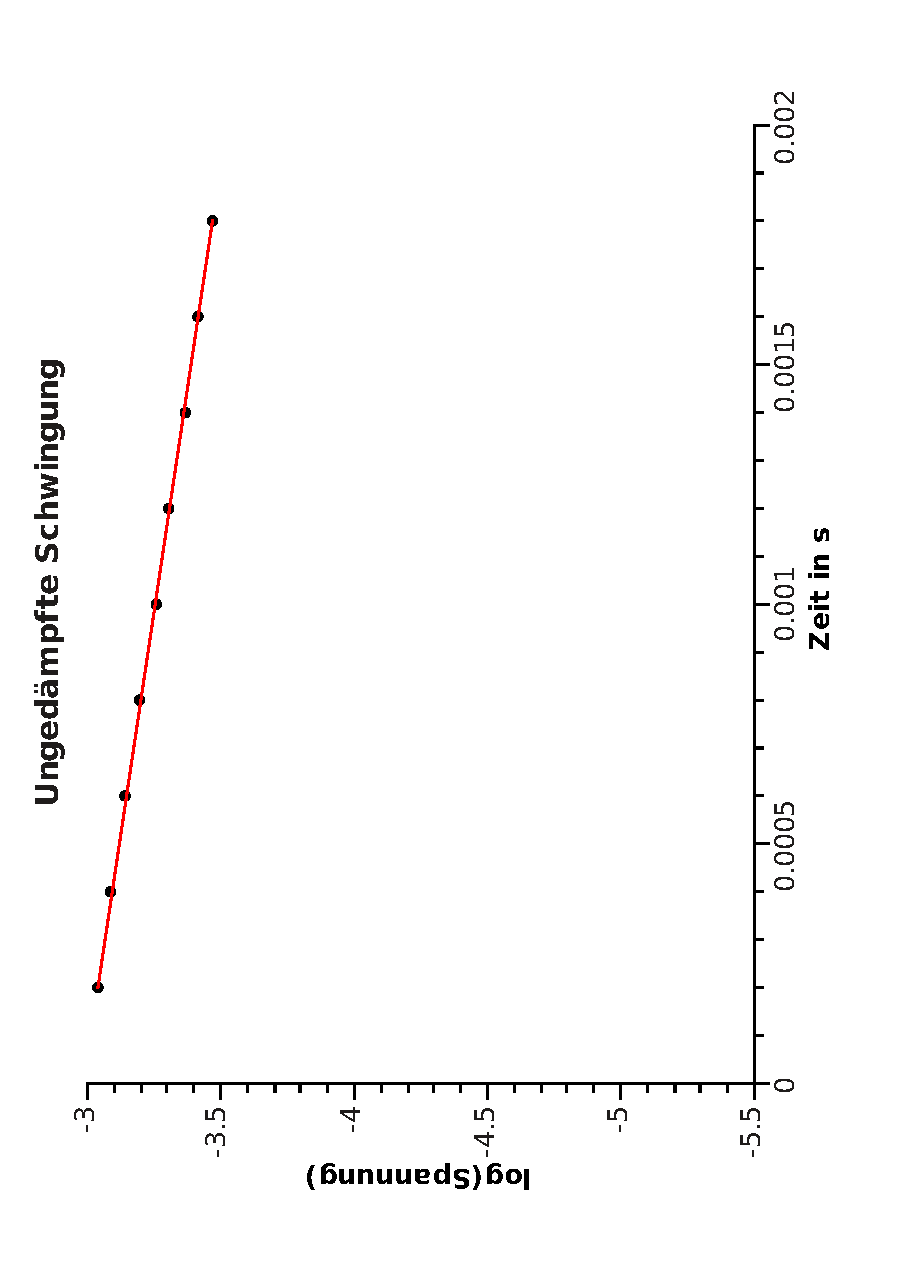
\includegraphics[width=0.9\linewidth ,angle=-90]{ungesing.eps}
\end{subfigure}
\begin{subfigure}{0.5\textwidth}
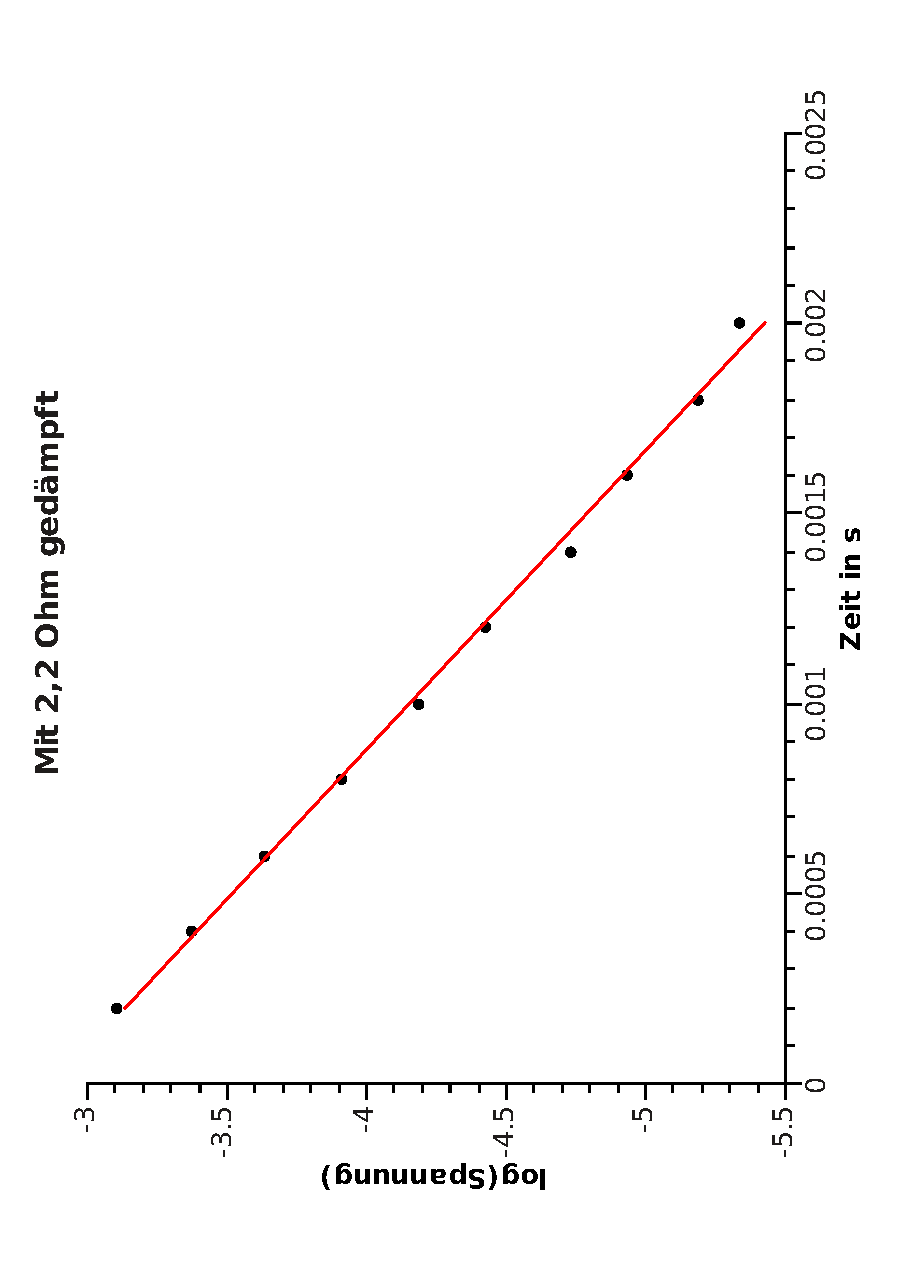
\includegraphics[width=0.9\linewidth ,angle=-90]{gesing.eps}
\end{subfigure}
\end{figure}
\begin{center}
\begin{figure}
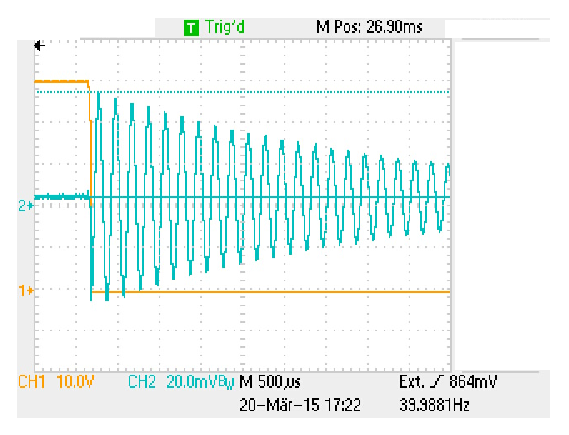
\includegraphics[width=0.5\linewidth]{freieschw.eps}
\end{figure}
\end{center}
\subsection*{Kapazität des Schwingkreises}
\label{Kapa}
Mit L=1.00$\pm$0.03 mH :\\
\subsubsection*{Ohne Dämpfung} 
\begin{center}C=(1.01$ \pm 0.04) \cdot 10^{-6}$F \end{center}
\subsubsection*{Mit Dämpfung}  
\begin{center}C=(1.01 $ \pm 0.04) \cdot 10^{-6}$F \end{center} 

\subsection*{Widerstand der Spule}


\subsubsection*{Ohne Dämpfung}
R=(0.54 $\pm0.02) \Omega$\\

\subsubsection*{Mit Dämpfung} 
R=(2.5 $\pm 0.1) \Omega$ \\


\subsection{Erzwungene Schwingungen}


\subsection*{Resonanzkurven}


\begin{center}
\begin{figure}
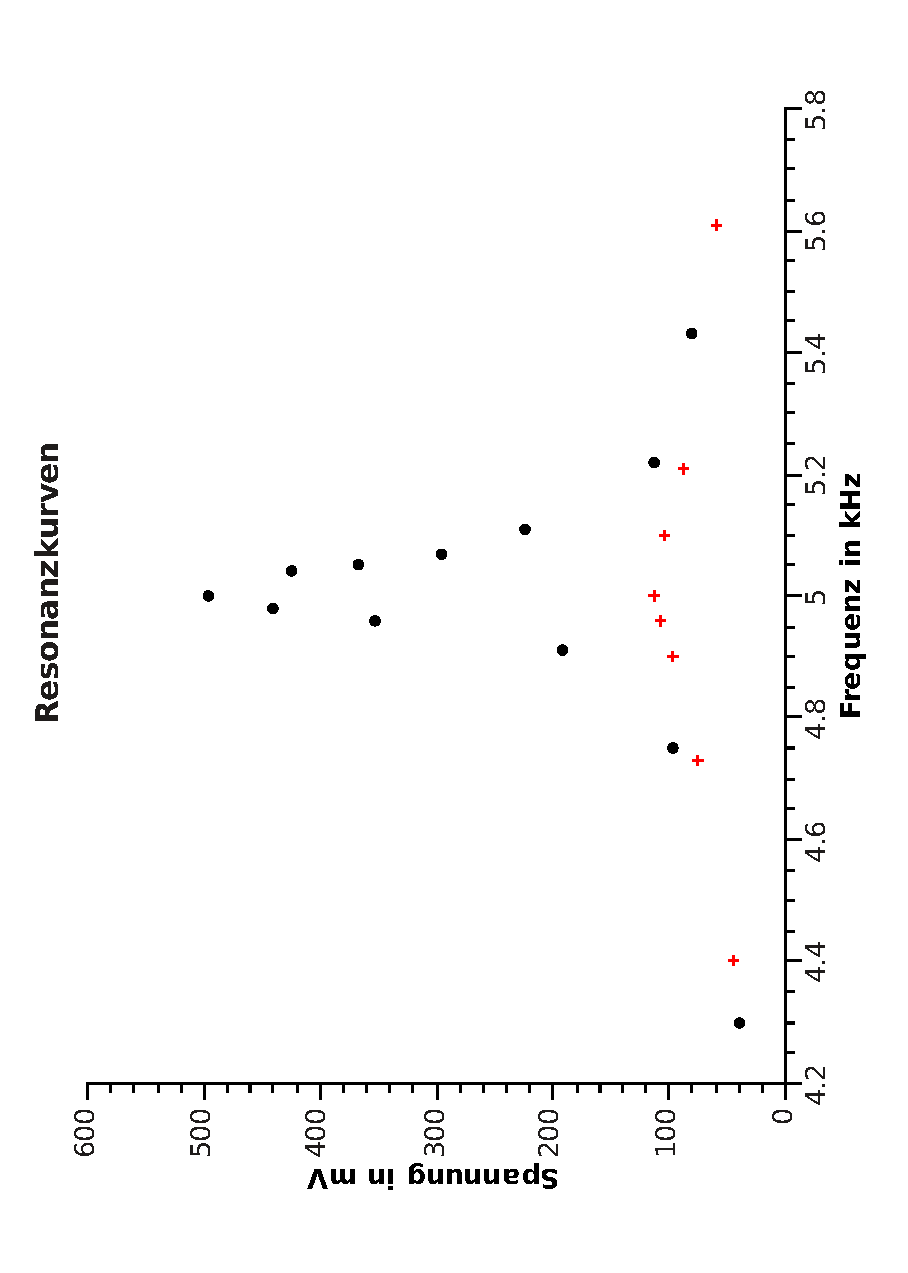
\includegraphics[width=0.5\linewidth ,angle=-90]{resonanzkurven.eps}
\caption{Resonanzkurven für die gedämpfte und die ungedämpfte erzwungene Schwingung}
\end{figure}
\end{center}

Resonanzfrequenz von genau 5kHz in beiden Fällen.

\subsection*{Phasenverschiebung}
\subsubsection*{Mit Dämpfung}
bei 0.8 $\omega_{max}$: $\pi$\\
bei $\omega_{max}$: $\pi$/2\\
bei 1.2 $\omega_{max}$: 0\\



\subsubsection*{Ohne Dämpfung}
bei 0.8 $\omega_{max}$: $\pi$\\
bei $\omega_{max}$: $\pi$/2\\
bei 1.2 $\omega_{max}$: 0\\

Die Phasenverschiebung dreht also wie erwartet von +$\pi$ auf 0.

\begin{figure}
\begin{subfigure}{0.3\textwidth}
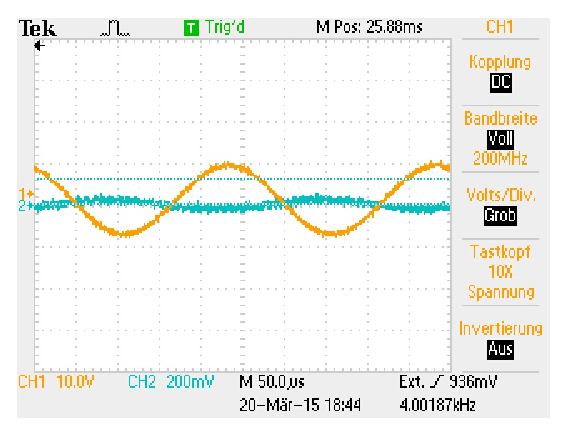
\includegraphics[width=0.9\linewidth ]{reso3.eps}
\caption{0.8 $\omega_{max}$}
\end{subfigure}
\begin{subfigure}{0.3\textwidth}
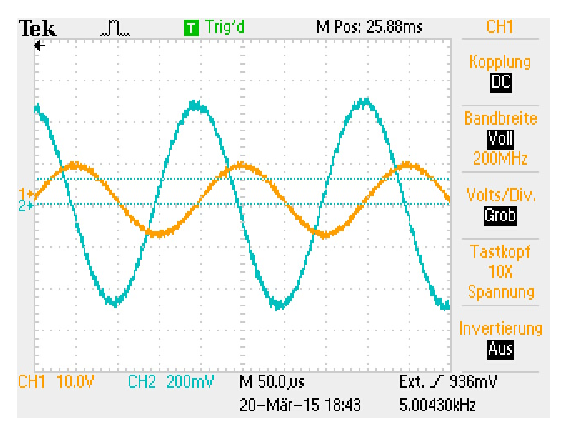
\includegraphics[width=0.9\linewidth]{reso2.eps}
\caption{1 $\omega_{max}$}
\end{subfigure}
\begin{subfigure}{0.3\textwidth}
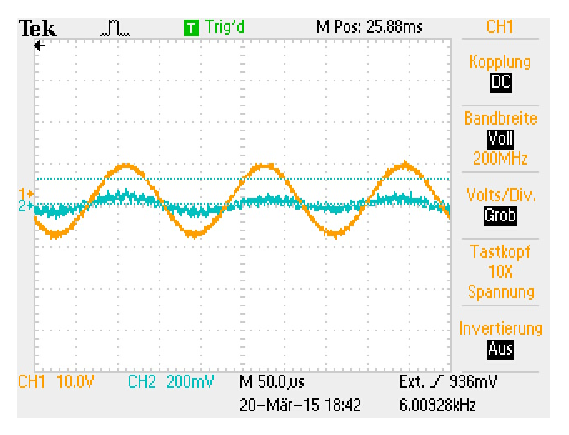
\includegraphics[width=0.9\linewidth]{reso1.eps}
\caption{1.2 $\omega_{max}$}
\end{subfigure}
\caption{Phasenverschiebungen}
\end{figure}

\subsection*{Eigenfrequenz, Dämpfung, Gütefaktor}
Durch die Breite der Resonanzkurve bei $\frac{1}{\sqrt{2}}$ des Maximums bestimmt:
\subsubsection*{Ohne Dämpfung}
$\delta \approx$0.05\\
Q$\approx$200
\subsubsection*{Mit Dämpfung}
$\delta \approx$0.3\\
Q$\approx$20
\subsection{Gekoppelte Schwingkreise}
%19.73Hz Triggerfrequenz, Rechteck

%Ein Bild mit ausgeschaltetem Kopplungskondensator
\begin{tabular}{c|c|c}
&3$\mu$F & 6$\mu$F \\
\hline $\omega_S$ & (1.45 $\pm$ 0.01) kHz & (760$\pm$ 10) Hz\\
$\omega_M$ & (5.88 $\pm$ 0.01) kHz & (5.26 $\pm$ 0.01) kHz\\
\end{tabular}\\

Aus den Kapazitäten berechnete Kopplungsgrade:\\
\begin{center}
3$\mu$F: K=0.25 $\pm$ 0.01 \\
6$\mu$F: K=0.14 $\pm$ 0.01
\end{center}
Aus den Frequenzen berechnete Kopplungsgrade:\\
\begin{center}
3$\mu$F: K=0.46 $\pm$ 0.01 \\
6$\mu$F: K=0.28 $\pm$ 0.01
\end{center}
\subsubsection*{Eigenfrequenzen}

Aus $\omega_S$ und $\omega_M$ berechnet:
\begin{tabular}{c|c|c}
&3 $\mu$F & 6 $\mu$F\\
\hline $\omega_{gegen}$ & (7.33 $\pm$ 0.01) kHz & (6.02 $\pm$ 0.01) kHz \\
$\omega_{gleich}$ & (4.43 $\pm$ 0.01) kHz & (4.50 $\pm$ 0.01) kHz \\
\end{tabular}\\
Gemessene Eigenfrequenzen:\\
\begin{center}
6 $\mu$F:\\
Schwingkreis 1:
(5002 $\pm$ 3) Hz\\
Schwingkreis 2:
(5021 $\pm$ 3) Hz\\
\vspace{0.5cm}
3$\mu$F:\\
Schwingkreis 1:(5000Hz $\pm$ 3)\\
Schwingkreis 2:(5027Hz $\pm$ 3)
\end{center}
\begin{center}
\begin{figure}
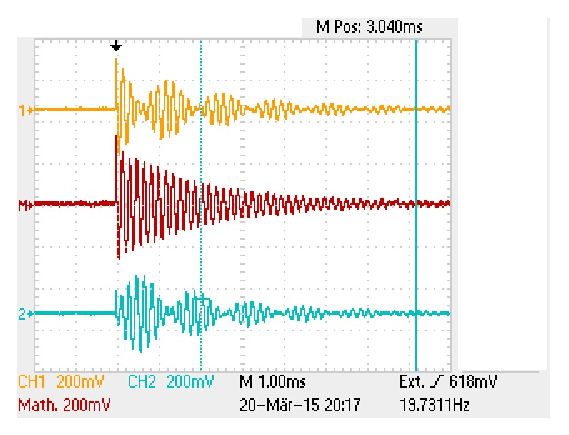
\includegraphics[width=0.5\linewidth]{reso.eps}
\end{figure}
\end{center}
\section{Diskussion}
\subsection{Freie Schwingungen}
Es ist genial wie wir durch die Betrachtung der Maxima der Schwingungsgleichung \ref{Schwingungsgleichung} den Cosinus in der Formel auf 1 setzen und nach $\delta$T umformen konnten, denn wenn wir einfach die Maxima der Schwingung am Oszilloskop ablesen, sie logarithmieren und gegen T auftragen erhalten wir $\delta$ als Steigung der Gerade! So können wir weiter einfach durch Vergleich mit der gemessenen Kreisfrequenz die Eigenfrequenz des Schwingkreises ermitteln. \\

Man erkennt in \ref{Kapa} dass die Dämpfung des Schwingkreises für seine Kapazität unbedeutend ist - der berechnete Unterschied liegt unterhalb der Messgenauigkeit!\\

Interessant war vor allem zu sehen wie genau der Schwingkreis mit dem Umpolen der Spannung durch das Rechtecksignal zu schwingen begann, und wie viel Energie er durch die Leitungswärme verlor - zu sehen an dem schnellen Abklingen.
\subsection{Erzwungene Schwingungen}
Verglichen mit der freien Schwingung hat die erzwungene einen doppelt bis vier mal so großen Gütefaktor, was auf die ständige Anregung der Schwingung zurückzuführen ist - man regt sie nicht nur einmal an und lässt sie ausklingen, sondern führt ihr ständig Energie zu. 
\subsection{Gekoppelte Schwingungen}
Es war sehr schön zu sehen wie die Enerige aus einem Schwingkreis in den nächsten wanderte und wieder zurück, und zwar über die Spannung, die sich am koppelnden Kondensator aufbaute. Sinnvollerweise entsprach einer höheren Kapazität des koppelnden Kondensators eine langsamere Schwebung, da er sich ja auch langsamer ladete. \\
Die Kopplungsgrade aus den Frequenzen stimmen nicht gut mit denen aus den Kapazitäten zusammen, ich finde aber keinen Fehler an deren Berechnung.
																			
\end{document}
